\documentclass[10pt]{article}
\usepackage[polish]{babel}
\usepackage[utf8]{inputenc}
\usepackage[T1]{fontenc}
\usepackage{graphicx}
\usepackage[export]{adjustbox}
\graphicspath{ {./images/} }
\usepackage{amsmath}
\usepackage{amsfonts}
\usepackage{amssymb}
\usepackage[version=4]{mhchem}
\usepackage{stmaryrd}

\title{EGZAMIN MATURALNY Z MATEMATYKI }

\author{}
\date{}


\begin{document}
\maketitle

\includegraphics[max width=\textwidth, center]{2024_11_21_4b04c3bb9b70693ba152g-01}\\
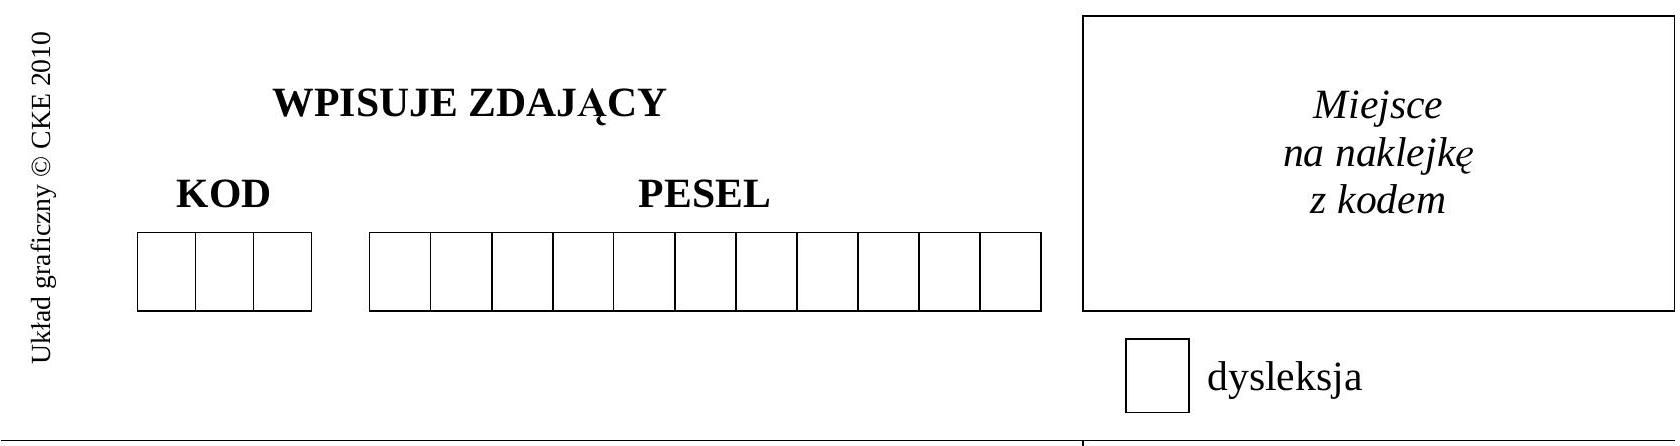
\includegraphics[max width=\textwidth, center]{2024_11_21_4b04c3bb9b70693ba152g-01(1)}

\section*{POZIOM PODSTAWOWY}
\begin{enumerate}
  \item Sprawdź, czy arkusz egzaminacyjny zawiera 18 stron (zadania 1-34). Ewentualny brak zgłoś przewodniczącemu zespołu nadzorującego egzamin.
  \item Rozwiąania zadań i odpowiedzi wpisuj w miejscu na to przeznaczonym.
  \item Odpowiedzi do zadań zamkniętych (1-24) przenieś na kartę odpowiedzi, zaznaczając je w części karty przeznaczonej dla zdającego. Zamaluj ■ pola do tego przeznaczone. Błędne zaznaczenie otocz kółkiem i zaznacz właściwe.
  \item Pamiętaj, że pominięcie argumentacji lub istotnych obliczeń w rozwiązaniu zadania otwartego (25-34) może spowodować, że za to rozwiązanie nie będziesz mógł
\end{enumerate}

CZERWIEC 2012 dostać pełnej liczby punktów.\\
5. Pisz czytelnie i używaj tylko długopisu lub pióra z czarnym tuszem lub atramentem.\\
6. Nie używaj korektora, a błędne zapisy wyraźnie przekreśl.\\
7. Pamiętaj, że zapisy w brudnopisie nie będą oceniane.\\
8. Możesz korzystać z zestawu wzorów matematycznych, cyrkla i linijki oraz kalkulatora.\\
9. Na tej stronie oraz na karcie odpowiedzi wpisz swój numer PESEL i przyklej naklejkę z kodem.\\
10. Nie wpisuj żadnych znaków w części przeznaczonej dla egzaminatora.

Czas pracy: 170 minut

Liczba punktów do uzyskania: 50

MMA-P1\_1P-123

\section*{ZADANIA ZAMKNIĘTE}
\section*{W zadaniach od 1. do 24. wybierz i zaznacz na karcie odpowiedzi poprawnq odpowiedź.}
\section*{Zadanie 1. (1 pkt)}
Ułamek \(\frac{\sqrt{5}+2}{\sqrt{5}-2}\) jest równy\\
A. 1\\
B. -1\\
C. \(7+4 \sqrt{5}\)\\
D. \(9+4 \sqrt{5}\)

\section*{Zadanie 2. (1 pkt)}
Liczbami spełniającymi równanie \(|2 x+3|=5\) są\\
A. \(1 \mathrm{i}-4\)\\
B. 1 i 2\\
C. -1 i 4\\
D. -2 i 2

\section*{Zadanie 3. (1 pkt)}
Równanie \((x+5)(x-3)\left(x^{2}+1\right)=0\) ma\\
A. dwa rozwiazania: \(x=-5, x=3\).\\
B. dwa rozwiązania: \(x=-3, x=5\).\\
C. cztery rozwiązania: \(x=-5, x=-1, x=1, x=3\).\\
D. cztery rozwiązania: \(x=-3, x=-1, x=1, x=5\).

\section*{Zadanie 4. (1 pkt)}
Marża równa 1,5\% kwoty pożyczonego kapitału była równa 3000 zł. Wynika stąd, że pożyczono\\
A. 45 zl\\
B. \(2000 \mathrm{zł}\)\\
C. \(200000 \mathrm{zł}\)\\
D. \(450000 \mathrm{zł}\)

\section*{Zadanie 5. (1 pkt)}
Na jednym z poniższych rysunków przedstawiono fragment wykresu funkcji \(y=x^{2}+2 x-3\). Wskaż ten rysunek.\\
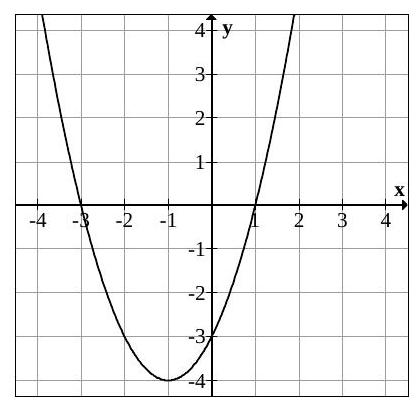
\includegraphics[max width=\textwidth, center]{2024_11_21_4b04c3bb9b70693ba152g-02(2)}\\
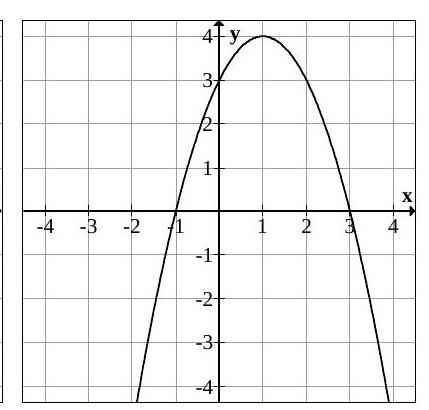
\includegraphics[max width=\textwidth, center]{2024_11_21_4b04c3bb9b70693ba152g-02(1)}\\
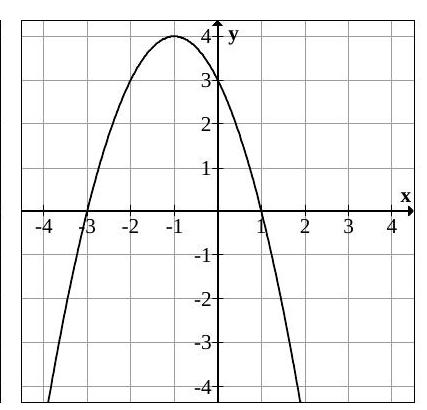
\includegraphics[max width=\textwidth, center]{2024_11_21_4b04c3bb9b70693ba152g-02}\\
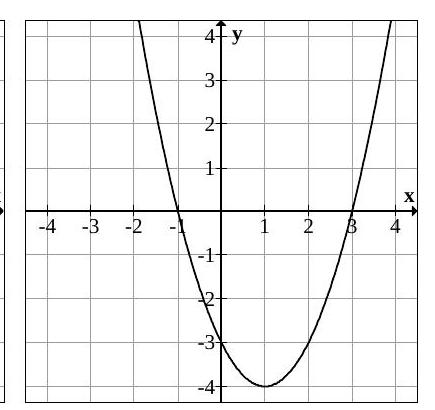
\includegraphics[max width=\textwidth, center]{2024_11_21_4b04c3bb9b70693ba152g-02(3)}\\
A.\\
B.\\
C.\\
D.\\

\includegraphics[max width=\textwidth, center]{2024_11_21_4b04c3bb9b70693ba152g-03}

\section*{Zadanie 6. (1 pkt)}
Wierzchołkiem paraboli będącej wykresem funkcji określonej wzorem \(f(x)=x^{2}-4 x+4\) jest punkt o współrzędnych\\
A. \((0,2)\)\\
B. \((0,-2)\)\\
C. \((-2,0)\)\\
D. \((2,0)\)

\section*{Zadanie 7. (1 pkt)}
Jeden kąt trójkąta ma miarę \(54^{\circ}\). Z pozostałych dwóch kątów tego trójkąta jeden jest 6 razy większy od drugiego. Miary pozostałych kątów są równe\\
A. \(21^{\circ} \mathrm{i} 105^{\circ}\)\\
B. \(11^{\circ}\) i \(66^{\circ}\)\\
C. \(18^{\circ}\) i \(108^{\circ}\)\\
D. \(16^{\circ}\) i \(96^{\circ}\)

\section*{Zadanie 8. (1 pkt)}
Krótszy bok prostokąta ma długość 6. Kąt między przekątną prostokąta i dłuższym bokiem ma miarę \(30^{\circ}\). Dłuższy bok prostokąta ma długość\\
A. \(2 \sqrt{3}\)\\
B. \(4 \sqrt{3}\)\\
C. \(6 \sqrt{3}\)\\
D. 12

\section*{Zadanie 9. (1 pkt)}
Cięciwa okręgu ma długość 8 cm i jest oddalona od jego środka o 3 cm . Promień tego okręgu ma długość\\
A. 3 cm\\
B. 4 cm\\
C. 5 cm\\
D. 8 cm

\section*{Zadanie 10. (1 pkt)}
Punkt \(O\) jest środkiem okręgu. Kąt wpisany \(B A D\) ma miarę\\
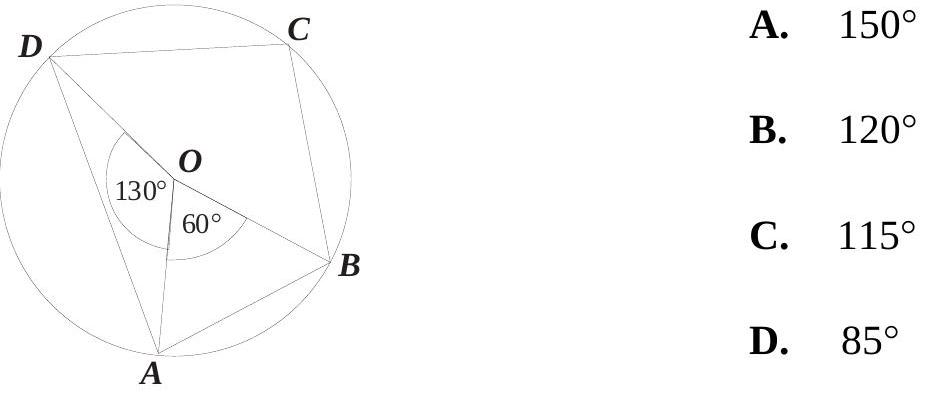
\includegraphics[max width=\textwidth, center]{2024_11_21_4b04c3bb9b70693ba152g-04}

\section*{Zadanie 11. (1 pkt)}
Pięciokąt \(A B C D E\) jest foremny. Wskaż trójkąt przystający do trójkąta \(E C D\)\\
D\\
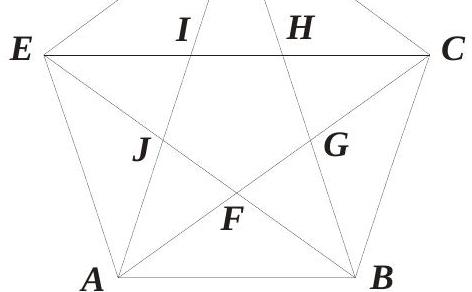
\includegraphics[max width=\textwidth, center]{2024_11_21_4b04c3bb9b70693ba152g-04(1)}\\
A. \(\triangle A B F\)\\
B. \(\triangle C A B\)\\
C. \(\triangle I H D\)\\
D. \(\triangle A B D\)\\

\includegraphics[max width=\textwidth, center]{2024_11_21_4b04c3bb9b70693ba152g-05}

\section*{Zadanie 12. (1 pkt)}
Punkt \(O\) jest środkiem okrequ przedstawionego na rysunku. Równanie tego okrequ ma postać:\\
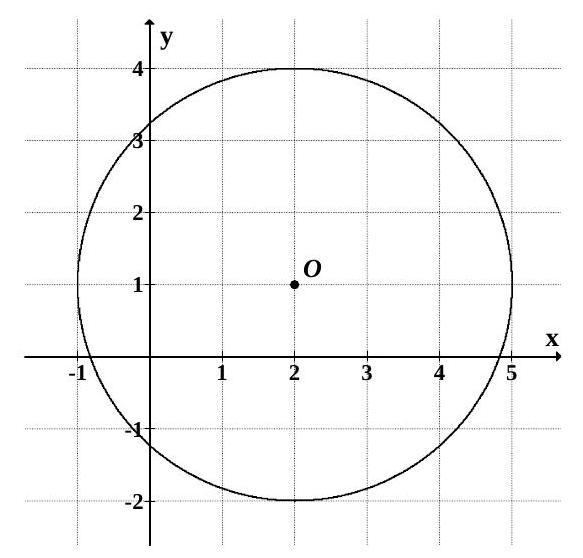
\includegraphics[max width=\textwidth, center]{2024_11_21_4b04c3bb9b70693ba152g-06}\\
A. \((x-2)^{2}+(y-1)^{2}=9\)\\
B. \((x-2)^{2}+(y-1)^{2}=3\)\\
C. \((x+2)^{2}+(y+1)^{2}=9\)\\
D. \((x+2)^{2}+(y+1)^{2}=3\)

\section*{Zadanie 13. (1 pkt)}
Wyrażenie \(\frac{3 x+1}{x-2}-\frac{2 x-1}{x+3}\) jest równe\\
A. \(\frac{x^{2}+15 x+1}{(x-2)(x+3)}\)\\
B. \(\frac{x+2}{(x-2)(x+3)}\)\\
C. \(\frac{x}{(x-2)(x+3)}\)\\
D. \(\frac{x+2}{-5}\)

\section*{Zadanie 14. (1 pkt)}
Ciagg \(\left(a_{n}\right)\) jest określony wzorem \(a_{n}=\sqrt{2 n+4}\) dla \(n \geq 1\). Wówczas\\
A. \(a_{8}=2 \sqrt{5}\)\\
B. \(a_{8}=8\)\\
C. \(a_{8}=5 \sqrt{2}\)\\
D. \(a_{8}=\sqrt{12}\)

\section*{Zadanie 15. (1 pkt)}
Ciag \((2 \sqrt{2}, 4, a)\) jest geometryczny. Wówczas\\
A. \(a=8 \sqrt{2}\)\\
B. \(a=4 \sqrt{2}\)\\
C. \(a=8-2 \sqrt{2}\)\\
D. \(a=8+2 \sqrt{2}\)

\section*{Zadanie 16. (1 pkt)}
Kąt \(\alpha\) jest ostry i \(\operatorname{tg} \alpha=1\). Wówczas\\
A. \(\alpha<30^{\circ}\)\\
B. \(\alpha=30^{\circ}\)\\
C. \(\alpha=45^{\circ}\)\\
D. \(\alpha>45^{\circ}\)

\section*{Zadanie 17. (1 pkt)}
Wiadomo, że dziedziną funkcji \(f\) określonej wzorem \(f(x)=\frac{x-7}{2 x+a}\) jest zbiór \((-\infty, 2) \cup(2,+\infty)\). Wówczas\\
A. \(a=2\)\\
B. \(a=-2\)\\
C. \(a=4\)\\
D. \(a=-4\)\\

\includegraphics[max width=\textwidth, center]{2024_11_21_4b04c3bb9b70693ba152g-07}

\section*{Zadanie 18. (1 pkt)}
Jeden z rysunków przedstawia wykres funkcji liniowej \(f(x)=a x+b\), gdzie \(a>0\) i \(b<0\). Wskaż ten wykres.\\
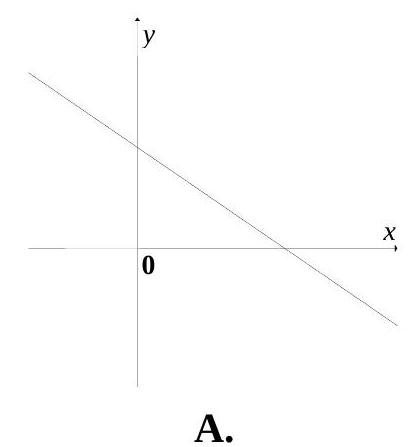
\includegraphics[max width=\textwidth, center]{2024_11_21_4b04c3bb9b70693ba152g-08(3)}\\
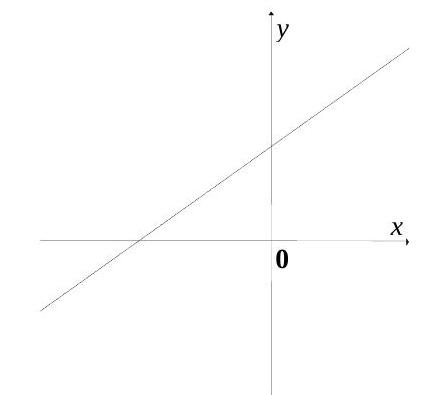
\includegraphics[max width=\textwidth, center]{2024_11_21_4b04c3bb9b70693ba152g-08(1)}\\
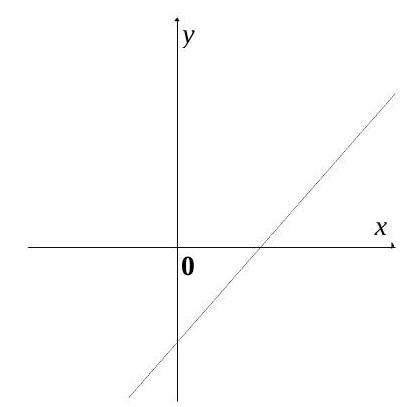
\includegraphics[max width=\textwidth, center]{2024_11_21_4b04c3bb9b70693ba152g-08(2)}\\
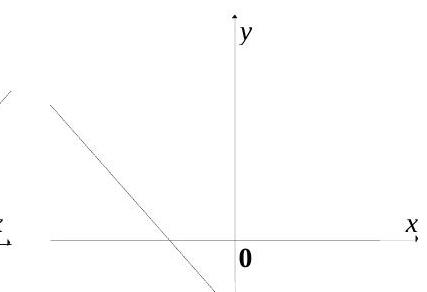
\includegraphics[max width=\textwidth, center]{2024_11_21_4b04c3bb9b70693ba152g-08}

Zadanie 19. (1 pkt)\\
Punkt \(S=(2,7)\) jest środkiem odcinka \(A B\), w którym \(A=(-1,3)\). Punkt \(B\) ma współrzędne:\\
A. \(B=(5,11)\)\\
B. \(\quad B=\left(\frac{1}{2}, 2\right)\)\\
C. \(B=\left(-\frac{3}{2},-5\right)\)\\
D. \(B=(3,11)\)

\section*{Zadanie 20. (1 pkt)}
W kolejnych sześciu rzutach kostką otrzymano następujące wyniki: 6, 3, 1, 2, 5, 5. Mediana tych wyników jest równa:\\
A. 3\\
B. 3,5\\
C. 4\\
D. 5

\section*{Zadanie 21. (1 pkt)}
Równość \((a+2 \sqrt{2})^{2}=a^{2}+28 \sqrt{2}+8\) zachodzi dla\\
A. \(a=14\)\\
B. \(a=7 \sqrt{2}\)\\
C. \(a=7\)\\
D. \(a=2 \sqrt{2}\)

\section*{Zadanie 22. (1 pkt)}
Trójkąt prostokątny o przyprostokątnych 4 i 6 obracamy wokół dłuższej przyprostokątnej. Objętość powstałego stożka jest równa\\
A. \(96 \pi\)\\
B. \(48 \pi\)\\
C. \(32 \pi\)\\
D. \(8 \pi\)

\section*{Zadanie 23. (1 pkt)}
Jeżeli \(A\) i \(B\) są zdarzeniami losowymi, \(B^{\prime}\) jest zdarzeniem przeciwnym do \(B, P(A)=0,3\), \(P\left(B^{\prime}\right)=0,4\) oraz \(A \cap B=\varnothing\), to \(P(A \cup B)\) jest równe\\
A. 0,12\\
B. 0,18\\
C. 0,6\\
D. 0,9

\section*{Zadanie 24. (1 pkt)}
Przekrój osiowy walca jest kwadratem o boku \(a\). Jeżeli \(r\) oznacza promień podstawy walca, h oznacza wysokość walca, to\\
A. \(r+h=a\)\\
B. \(h-r=\frac{a}{2}\)\\
C. \(r-h=\frac{a}{2}\)\\
D. \(r^{2}+h^{2}=a^{2}\)\\

\includegraphics[max width=\textwidth, center]{2024_11_21_4b04c3bb9b70693ba152g-09}

\section*{ZADANIA OTWARTE}
\section*{Rozwiqzania zadań o numerach od 25. do 34. należy zapisać w wyznaczonych miejscach pod treściq zadania.}
\section*{Zadanie 25. (2 pkt)}
Rozwiąż nierówność \(x^{2}-3 x-10<0\).

\begin{center}
\begin{tabular}{|c|c|c|c|c|c|c|c|c|c|c|c|c|c|c|c|c|c|c|c|c|c|c|c|c|c|c|c|c|c|c|c|}
\hline
 &  &  &  &  &  &  &  &  &  &  &  &  &  &  &  &  &  &  &  &  &  &  &  &  &  &  &  &  &  &  &  \\
\hline
 &  &  &  &  &  &  &  &  &  &  &  &  &  &  &  &  &  &  &  &  &  &  &  &  &  &  &  &  &  &  &  \\
\hline
 &  &  &  &  &  &  &  &  &  &  &  &  &  &  &  &  &  &  &  &  &  &  &  &  &  &  &  &  &  &  &  \\
\hline
 &  &  &  &  &  &  &  &  &  &  &  &  &  &  &  &  &  &  &  &  &  &  &  &  &  &  &  &  &  &  &  \\
\hline
 &  &  &  &  &  &  &  &  &  &  &  &  &  &  &  &  &  &  &  &  &  &  &  &  &  &  &  &  &  &  &  \\
\hline
 &  &  &  &  &  &  &  &  &  &  &  &  &  &  &  &  &  &  &  &  &  &  &  &  &  &  &  &  &  &  &  \\
\hline
 &  &  &  &  &  &  &  &  &  &  &  &  &  &  &  &  &  &  &  &  &  &  &  &  &  &  &  &  &  &  &  \\
\hline
 &  &  &  &  &  &  &  &  &  &  &  &  &  &  &  &  &  &  &  &  &  &  &  &  &  &  &  &  &  &  &  \\
\hline
 &  &  &  &  &  &  &  &  &  &  &  &  &  &  &  &  &  &  &  &  &  &  &  &  &  &  &  &  &  &  &  \\
\hline
 &  &  &  &  &  &  &  &  &  &  &  &  &  &  &  &  &  &  &  &  &  &  &  &  &  &  &  &  &  &  &  \\
\hline
 &  &  &  &  &  &  &  &  &  &  &  &  &  &  &  &  &  &  &  &  &  &  &  &  &  &  &  &  &  &  &  \\
\hline
 &  &  &  &  &  &  &  &  &  &  &  &  &  &  &  &  &  &  &  &  &  &  &  &  &  &  &  &  &  &  &  \\
\hline
 &  &  &  &  &  &  &  &  &  &  &  &  &  &  &  &  &  &  &  &  &  &  &  &  &  &  &  &  &  &  &  \\
\hline
 &  &  &  &  &  &  &  &  &  &  &  &  &  &  &  &  &  &  &  &  &  &  &  &  &  &  &  &  &  &  &  \\
\hline
 &  &  &  &  &  &  &  &  &  &  &  &  &  &  &  &  &  &  &  &  &  &  &  &  &  &  &  &  &  &  &  \\
\hline
 &  &  &  &  &  &  &  &  &  &  &  &  &  &  &  &  &  &  &  &  &  &  &  &  &  &  &  &  &  &  &  \\
\hline
 &  &  &  &  &  &  &  &  &  &  &  &  &  &  &  &  &  &  &  &  &  &  &  &  &  &  &  &  &  &  &  \\
\hline
\end{tabular}
\end{center}

Odpowiedź:

\section*{Zadanie 26. (2 pkt)}
Średnia wieku w pewnej grupie studentów jest równa 23 lata. Średnia wieku tych studentów i ich opiekuna jest równa 24 lata. Opiekun ma 39 lat. Oblicz, ilu studentów jest w tej grupie.

\begin{center}
\begin{tabular}{|c|c|c|c|c|c|c|c|c|c|c|c|c|c|c|c|c|c|c|c|c|c|c|c|c|c|c|c|c|c|c|}
\hline
 &  &  &  &  &  &  &  &  &  &  &  &  &  &  &  &  &  &  &  &  &  &  &  &  &  &  &  &  &  &  \\
\hline
 &  &  &  &  &  &  &  &  &  &  &  &  &  &  &  &  &  &  &  &  &  &  &  &  &  &  &  &  &  &  \\
\hline
 &  &  &  &  &  &  &  &  &  &  &  &  &  &  &  &  &  &  &  &  &  &  &  &  &  &  &  &  &  &  \\
\hline
 &  &  &  &  &  &  &  &  &  &  &  &  &  &  &  &  &  &  &  &  &  &  &  &  &  &  &  &  &  &  \\
\hline
 &  &  &  &  &  &  &  &  &  &  &  &  &  &  &  &  &  &  &  &  &  &  &  &  &  &  &  &  &  &  \\
\hline
 &  &  &  &  &  &  &  &  &  &  &  &  &  &  &  &  &  &  &  &  &  &  &  &  &  &  &  &  &  &  \\
\hline
 &  &  &  &  &  &  &  &  &  &  &  &  &  &  &  &  &  &  &  &  &  &  &  &  &  &  &  &  &  &  \\
\hline
 &  &  &  &  &  &  &  &  &  &  &  &  &  &  &  &  &  &  &  &  &  &  &  &  &  &  &  &  &  &  \\
\hline
 &  &  &  &  &  &  &  &  &  &  &  &  &  &  &  &  &  &  &  &  &  &  &  &  &  &  &  &  &  &  \\
\hline
 &  &  &  &  &  &  &  &  &  &  &  &  &  &  &  &  &  &  &  &  &  &  &  &  &  &  &  &  &  &  \\
\hline
 &  &  &  &  &  &  &  &  &  &  &  &  &  &  &  &  &  &  &  &  &  &  &  &  &  &  &  &  &  &  \\
\hline
 &  &  &  &  &  &  &  &  &  &  &  &  &  &  &  &  &  &  &  &  &  &  &  &  &  &  &  &  &  &  \\
\hline
 &  &  &  &  &  &  &  &  &  &  &  &  &  &  &  &  &  &  &  &  &  &  &  &  &  &  &  &  &  &  \\
\hline
 &  &  &  &  &  &  &  &  &  &  &  &  &  &  &  &  &  &  &  &  &  &  &  &  &  &  &  &  &  &  \\
\hline
 &  &  &  &  &  &  &  &  &  &  &  &  &  &  &  &  &  &  &  &  &  &  &  &  &  &  &  &  &  &  \\
\hline
 &  &  &  &  &  &  &  &  &  &  &  &  &  &  &  &  &  &  &  &  &  &  &  &  &  &  &  &  &  &  \\
\hline
 &  &  &  &  &  &  &  &  &  &  &  &  &  &  &  &  &  &  &  &  &  &  &  &  &  &  & 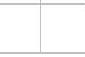
\includegraphics[max width=\textwidth]{2024_11_21_4b04c3bb9b70693ba152g-10}
 &  &  &  \\
\hline
\end{tabular}
\end{center}

Odpowiedź: \(\qquad\)

Zadanie 27. (2 pkt)\\
Podstawy trapezu prostokątnego mają długości 6 i 10 oraz tangens jego kąta ostrego jest równy 3. Oblicz pole tego trapezu.\\

\includegraphics[max width=\textwidth, center]{2024_11_21_4b04c3bb9b70693ba152g-11(1)}

Odpowiedź:

\section*{Zadanie 28. (2 pkt)}
Uzasadnij, że jeżeli \(\alpha\) jest kątem ostrym, to \(\sin ^{4} \alpha+\cos ^{2} \alpha=\sin ^{2} \alpha+\cos ^{4} \alpha\).\\

\includegraphics[max width=\textwidth, center]{2024_11_21_4b04c3bb9b70693ba152g-11}

\section*{Zadanie 29. (2 pkt)}
Uzasadnij, że suma kwadratów trzech kolejnych liczb całkowitych przy dzieleniu przez 3 daje resztę 2.

\begin{center}
\begin{tabular}{|c|c|c|c|c|c|c|c|c|c|c|c|c|c|c|c|c|c|c|c|c|c|c|c|c|c|}
\hline
 &  &  &  &  &  &  &  &  &  &  &  &  &  &  &  &  &  &  &  &  &  &  &  &  &  \\
\hline
 &  &  &  &  &  &  &  &  &  &  &  &  &  &  &  &  &  &  &  &  &  &  &  &  &  \\
\hline
 &  &  &  &  &  &  &  &  &  &  &  &  &  &  &  &  &  &  &  &  &  &  &  &  &  \\
\hline
 &  &  &  &  &  &  &  &  &  &  &  &  &  &  &  &  &  &  &  &  &  &  &  &  &  \\
\hline
 &  &  &  &  &  &  &  &  &  &  &  &  &  &  &  &  &  &  &  &  &  &  &  &  &  \\
\hline
 &  &  &  &  &  &  &  &  &  &  &  &  &  &  &  &  &  &  &  &  &  &  &  &  &  \\
\hline
 &  &  &  &  &  &  &  &  &  &  &  &  &  &  &  &  &  &  &  &  &  &  &  &  &  \\
\hline
 &  &  &  &  &  &  &  &  &  &  &  &  &  &  &  &  &  &  &  &  &  &  &  &  &  \\
\hline
 &  &  &  &  &  &  &  &  &  &  &  &  &  &  &  &  &  &  &  &  &  &  &  &  &  \\
\hline
 &  &  &  &  &  &  &  &  &  &  &  &  &  &  &  &  &  &  &  &  &  &  &  &  &  \\
\hline
 &  &  &  &  &  &  &  &  &  &  &  &  &  &  &  &  &  &  &  &  &  &  &  &  &  \\
\hline
 &  &  &  &  &  &  &  &  &  &  &  &  &  &  &  &  &  &  &  &  &  &  &  &  &  \\
\hline
 &  &  &  &  &  &  &  &  &  &  &  &  &  &  &  &  &  &  &  &  &  &  &  &  &  \\
\hline
 &  &  &  &  &  &  &  &  &  &  &  &  &  &  &  &  &  &  &  &  &  &  &  &  &  \\
\hline
 &  &  &  &  &  &  &  &  &  &  &  &  &  &  &  &  &  &  &  &  &  &  &  &  &  \\
\hline
 &  &  &  &  &  &  &  &  &  &  &  &  &  &  &  &  &  &  &  &  &  &  &  &  &  \\
\hline
 &  &  &  &  &  &  &  &  &  &  &  &  &  &  &  &  &  &  &  &  &  &  &  &  &  \\
\hline
\end{tabular}
\end{center}

\section*{Zadanie 30. (2 pkt)}
Suma \(S_{n}=a_{1}+a_{2}+\ldots+a_{n}\) początkowych \(n\) wyrazów pewnego ciagu arytmetycznego \(\left(a_{n}\right)\) jest określona wzorem \(S_{n}=n^{2}-2 n\) dla \(n \geq 1\). Wyznacz wzór na \(n\)-ty wyraz tego ciagu.\\

\includegraphics[max width=\textwidth, center]{2024_11_21_4b04c3bb9b70693ba152g-12}

Odpowiedź:

Zadanie 31. (2 pkt)\\
Dany jest romb, którego kąt ostry ma miarę \(45^{\circ}\), a jego pole jest równe \(50 \sqrt{2}\). Oblicz wysokość tego rombu.\\

\includegraphics[max width=\textwidth, center]{2024_11_21_4b04c3bb9b70693ba152g-13}

\section*{Zadanie 32. (4 pkt)}
Punkty \(A=(2,11), B=(8,23), C=(6,14)\) są wierzchołkami trójkąta. Wysokość trójkąta poprowadzona z wierzchołka \(C\) przecina prostą \(A B\) w punkcie \(D\). Oblicz współzędne punktu \(D\).

\begin{center}
\begin{tabular}{|c|c|c|c|c|c|c|c|c|c|c|c|c|c|c|c|c|c|c|c|c|c|c|c|}
\hline
 &  &  &  &  &  &  &  &  &  &  &  &  &  &  &  &  &  &  &  &  &  &  &  \\
\hline
 &  &  &  &  &  &  &  &  &  &  &  &  &  &  &  &  &  &  &  &  &  &  &  \\
\hline
 &  &  &  &  &  &  &  &  &  &  &  &  &  &  &  &  &  &  &  &  &  &  &  \\
\hline
 &  &  &  &  &  &  &  &  &  &  &  &  &  &  &  &  &  &  &  &  &  &  &  \\
\hline
 &  &  &  &  &  &  &  &  &  &  &  &  &  &  &  &  &  &  &  &  &  &  &  \\
\hline
 &  &  &  &  &  &  &  &  &  &  &  &  &  &  &  &  &  &  &  &  &  &  &  \\
\hline
 &  &  &  &  &  &  &  &  &  &  &  &  &  &  &  &  &  &  &  &  &  &  &  \\
\hline
 &  &  &  &  &  &  &  &  &  &  &  &  &  &  &  &  &  &  &  &  &  &  &  \\
\hline
 &  &  &  &  &  &  &  &  &  &  &  &  &  &  &  &  &  &  &  &  &  &  &  \\
\hline
 &  &  &  &  &  &  &  &  &  &  &  &  &  &  &  &  &  &  &  &  &  &  &  \\
\hline
 &  &  &  &  &  &  &  &  &  &  &  &  &  &  &  &  &  &  &  &  &  &  &  \\
\hline
 &  &  &  &  &  &  &  &  &  &  &  &  &  &  &  &  &  &  &  &  &  &  &  \\
\hline
 &  &  &  &  &  &  &  &  &  &  &  &  &  &  &  &  &  &  &  &  &  &  &  \\
\hline
 &  &  &  &  &  &  &  &  &  &  &  &  &  &  &  &  &  &  &  &  &  &  &  \\
\hline
 &  &  &  &  &  &  &  &  &  &  &  &  &  &  &  &  &  &  &  &  &  &  &  \\
\hline
 &  &  &  &  &  &  &  &  &  &  &  &  &  &  &  &  &  &  &  &  &  &  &  \\
\hline
 &  &  &  &  &  &  &  &  &  &  &  &  &  &  &  &  &  &  &  &  &  &  &  \\
\hline
 &  &  &  &  &  &  &  &  &  &  &  &  &  &  &  &  &  &  &  &  &  &  &  \\
\hline
 &  &  &  &  &  &  &  &  &  &  &  &  &  &  &  &  &  &  &  &  &  &  &  \\
\hline
 &  &  &  &  &  &  &  &  &  &  &  &  &  &  &  &  &  &  &  &  &  &  &  \\
\hline
 &  &  &  &  &  &  &  &  &  &  &  &  &  &  &  &  &  &  &  &  &  &  &  \\
\hline
 &  &  &  &  &  &  &  &  &  &  &  &  &  &  &  &  &  &  &  &  &  &  &  \\
\hline
 &  &  &  &  &  &  &  &  &  &  &  &  &  &  &  &  &  &  &  &  &  &  &  \\
\hline
 &  &  &  &  &  &  &  &  &  &  &  &  &  &  &  &  &  &  &  &  &  &  &  \\
\hline
 &  &  &  &  &  &  &  &  &  &  &  &  &  &  &  &  &  &  &  &  &  &  &  \\
\hline
 &  &  &  &  &  &  &  &  &  &  &  &  &  &  &  &  &  &  &  &  &  &  &  \\
\hline
 &  &  &  &  &  &  &  &  &  &  &  &  &  &  &  &  &  &  &  &  &  &  &  \\
\hline
 &  &  &  &  &  &  &  &  &  &  &  &  &  &  &  &  &  &  &  &  &  &  &  \\
\hline
 &  &  &  &  &  &  &  &  &  &  &  &  &  &  &  &  &  &  &  &  &  &  &  \\
\hline
 &  &  &  &  &  &  &  &  &  &  &  &  &  &  &  &  &  &  &  &  &  &  &  \\
\hline
 &  &  &  &  &  &  &  &  &  &  &  &  &  &  &  &  &  &  &  &  &  &  &  \\
\hline
 &  &  &  &  &  &  &  &  &  &  &  &  &  &  &  &  &  &  &  &  &  &  &  \\
\hline
 &  &  &  &  &  &  &  &  &  &  &  &  &  &  &  &  &  &  &  &  &  &  &  \\
\hline
 &  &  &  &  &  &  &  &  &  &  &  &  &  &  &  &  &  &  &  &  &  &  &  \\
\hline
 &  &  &  &  &  &  &  &  &  &  &  &  &  &  &  &  &  &  &  &  &  &  &  \\
\hline
 &  &  &  &  &  &  &  &  &  &  &  &  &  &  &  &  &  &  &  &  &  &  &  \\
\hline
 &  &  &  &  &  &  &  &  &  &  &  &  &  &  &  &  &  &  &  &  &  &  &  \\
\hline
 &  &  &  &  &  &  &  &  &  &  &  &  &  &  &  &  &  &  &  &  &  &  &  \\
\hline
 &  &  &  &  &  &  &  &  &  &  &  &  &  &  &  &  &  &  &  &  &  &  &  \\
\hline
 &  &  &  &  &  &  &  &  &  &  &  &  &  &  &  &  &  &  &  &  &  &  &  \\
\hline
 &  &  &  &  &  &  &  &  &  &  &  &  &  &  &  &  &  &  &  &  &  &  &  \\
\hline
 &  &  &  &  &  &  &  &  &  &  &  &  &  &  &  &  &  &  &  &  &  &  &  \\
\hline
 &  &  &  &  &  &  &  &  &  &  &  &  &  &  &  &  &  &  &  &  &  &  &  \\
\hline
\end{tabular}
\end{center}

Odpowiedź:

Zadanie 33. (4 pkt)\\
Oblicz, ile jest liczb naturalnych pięciocyfrowych, w zapisie których nie występuje zero, jest dokładnie jedna cyfra 7 i dokładnie jedna cyfra parzysta.\\

\includegraphics[max width=\textwidth, center]{2024_11_21_4b04c3bb9b70693ba152g-15}

Odpowiedź:

\section*{Zadanie 34. (4 pkt)}
Dany jest graniastosłup prawidłowy trójkątny \(A B C D E F\) o podstawach \(A B C\) i \(D E F\) i krawędziach bocznych \(A D, B E\) i \(C F\) (zobacz rysunek). Długość krawędzi podstawy \(A B\) jest równa 8, a pole trójkąta \(A B F\) jest równe 52. Oblicz objętość tego graniastosłupa.\\

\includegraphics[max width=\textwidth, center]{2024_11_21_4b04c3bb9b70693ba152g-16}\\

\includegraphics[max width=\textwidth, center]{2024_11_21_4b04c3bb9b70693ba152g-17}

Odpowiedź:

\section*{BRUDNOPIS}

\end{document}